\section{Introduction} \label{sec:introduction}

\begin{figure}[t]
  \centering

  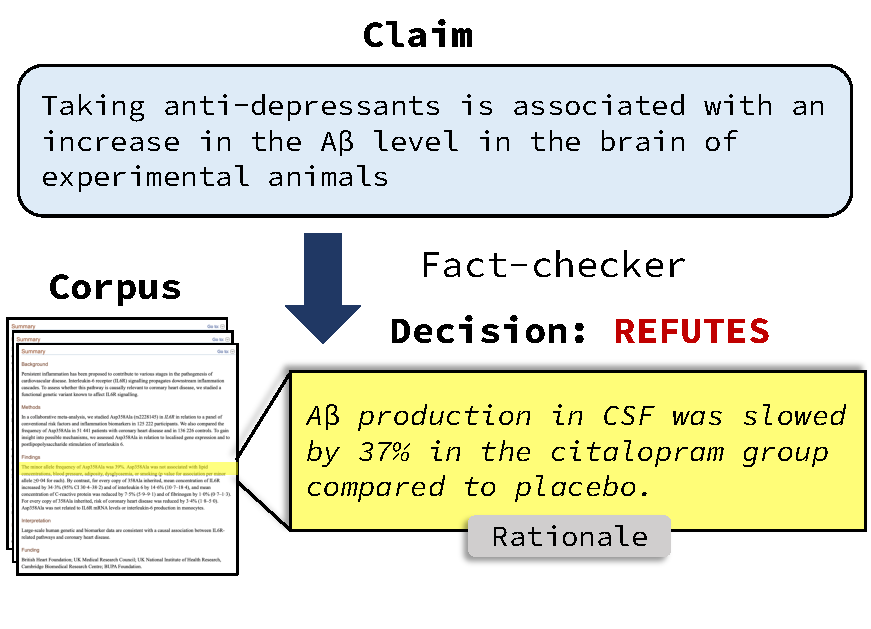
\includegraphics[width=\columnwidth]{figures/teaser-fig.pdf}
  \caption{A \ours claim refuted by evidence. To refute this claim, the system must recognize that (1) ``CSF'' is an acronym for ``cerebral spinal fluid'', found in the brain, (2) ``Citalopram'' is a type of antidepressant, but ``placebo'' is not, and (3) ``Slowing by 37\%'' indicates a reversal in effect relative to the claim.}
  \label{fig:teaser}
\end{figure}

\emph{Fact-checking} -- a task in which the veracity of an input \emph{claim} is verified against a corpus of documents that \emph{support} or \emph{refute} the claim -- has seen increased attention as an important research area. This attention is motivated by the proliferation of misinformation in political news, social media, and on the web \hanna{add citations}. In turn, interest in fact-checking has spurred the creation of many datasets across different domains to support research and development of automated fact-checking systems \hanna{add citations}.
Yet, to our knowledge, no such dataset exists to facilitate research on another important domain for fact-checking -- scientific literature. The ability to verify claims about scientific concepts, especially those related to biomedicine, is an important application area for fact-checking.  Furthermore, this line of research also offers a unique opportunity to explore the capabilities of modern neural models, since
successfully verifying most scientific claims requires expert background knowledge, complex language understanding, and reasoning capability, as demonstrated in Figure \ref{fig:teaser} and Table \ref{tbl:covid_example}.

% TODO(dwadden) bring back table of examples.
% % Some commands for colors and symbols.

\newcommand{\lexical}[1]{{\color{c1} \textbf{#1}}}
\newcommand{\numerical}[1]{{\color{c2} \textbf{#1}}}
\newcommand{\coref}[1]{{\color{c3} \textbf{#1}}}

%%%%%%%%%%%%%%%%%%%%

\begin{table*}[t]
  \setlength{\tabcolsep}{.25em}
  \footnotesize
  \centering

  \begin{subtable}[t!]{\linewidth}
    \begin{tabularx}{\textwidth}{ X l l l }
      \toprule
      \textbf{Claim} & \textbf{Association type} & \textbf{Causal} & \textbf{Directional} \\
      \midrule
      Female carriers of the Apolipoprotein E4 (APOE4) allele have a reduced risk for Alzheimer's disease. & Mutation / Disease & \xmark & \cmark \\
      \midrule
      Side effects associated with antidepressants increases risk of mortality in postmenopausal women. & Drug / Outcome & \cmark & \cmark \\
      \midrule
      Phosphorylation of the ATM protein regulates DNA damage-induced neuronal death. & Pathway / Phenotype & \cmark & \xmark \\
      \midrule
      Tuberculosis incidence is correlated with residential crowding in the UK. & Environment / Disease & \xmark & \cmark \\
      \bottomrule
    \end{tabularx}

    \subcaption{Claims express diverse associations; some are causal and / or directional.}
    \label{tbl:scifact_claim_types}
  \end{subtable}

  %%%%%%%%%%%%%%%%%%%%

  \begin{subtable}[t]{\linewidth} 

    \begin{tabularx}{\textwidth}{ X X r }
      \toprule
      \textbf{Claim} & \textbf{Evidence} & \textbf{Label} \\
      \midrule

      Taking \lexical{antidepressants} is associated with an increase in the A$\beta$ level in the brain of experimental animals. &
      A$\beta$ production in CSF was \numerical{slowed by 37\%} in the \lexical{citalopram} group compared to placebo. &
      \refutes \\
      \midrule

      Radiographic verified pneumonia predictions are improved by the combination of physical examinations with \lexical{C-reactive protein values}. &
      Addition of \lexical{CRP} at the \numerical{optimal cut off of $>$30 mg/L} increased the \numerical{ROC area to 0.77 (0.73 to 0.81)} \dots &
      \supports \\
      \midrule

      \coref{Low saturated fat diets} do not have adverse effects on growth or development of infants. &
      Neurological development of children in the \coref{intervention group} was at least as good as that of children in the control group. &
      \supports \\
      \midrule

      \lexical{Genomic instability} in leukemia cells results from a decrease in reactive oxygen species from oncogene activation. &
      BCR/ABL-induced reactive oxygen species (ROSs) cause \lexical{chronic oxidative DNA damage} \dots &
      \refutes \\

      \bottomrule
    \end{tabularx}

    \subcaption{The fact-checking system must recognize \lexical{lexical relations}, perform \numerical{quantitative reasoning} and \coref{coreference} resolution.}
    \label{tbl:scifact_reasoning_types}
  \end{subtable}

  \caption{Examples of common challenges unique to scientific fact-checking.}
  \label{tbl:scifact_challenges}
\end{table*}

\definecolor{c1}{RGB}{84,130,53}
% \newcommand{\supportsCovid}[1]{{\color{c1} \textbf{#1}}}
\newcommand{\supportsCovid}[1]{{\color{c1} {#1}}}

\definecolor{c2}{RGB}{218,0,0}
% \newcommand{\refutesCovid}[1]{{\color{c2} \textbf{#1}}}
\newcommand{\refutesCovid}[1]{{\color{c2} {#1}}}

\definecolor{c3}{RGB}{127,127,127}
\newcommand{\wrongContext}[1]{{\color{c3} \textbf{#1}}}



\begin{table*}[t!]
  \setlength{\tabcolsep}{.25em}
  \footnotesize
  \centering

  \begin{tabularx}{\textwidth}{ X }
    \toprule
    \textbf{Claim 1}: Lopinavir / ritonavir have exhibited favorable clinical responses when used as a treatment for coronavirus. \\
    \midrule
    \textbf{Supports}: \dots \supportsCovid{Interestingly, after lopinavir/ritonavir (Kaletra, AbbVie) was administered, $\beta$-coronavirus viral loads significantly decreased and no or little coronavirus titers were observed.} \\
    \midrule
    \textbf{Refutes}: \refutesCovid{The focused drug repurposing of known approved drugs (such as lopinavir/ritonavir) has been reported failed for curing SARS-CoV-2 infected patients.}. It is urgent to generate new chemical entities against this virus \dots \\
    \midrule
    \textbf{Claim 2}: The coronavirus cannot thrive in warmer climates. \\
    \midrule
    \textbf{Supports}: \supportsCovid{...most outbreaks display a pattern of clustering in relatively cool and dry areas...This is because the environment can mediate human-to-human transmission of SARS-CoV-2, and unsuitable climates can cause the virus to destabilize quickly...} \\
    \midrule
    \textbf{Refutes}: \refutesCovid{...significant cases in the coming months are likely to occur in more humid (warmer) climates, irrespective of the climate-dependence of transmission and that summer temperatures will not substrantially limit pandemic growth}. \\
    \bottomrule
  \end{tabularx}

  \caption{Evidence identified by our system as supporting and refuting two claims concerning COVID-19.}
  \label{tbl:covid_example}


\end{table*}


In this paper, we introduce the task of scientific fact-checking. To facilitate research on this task, we construct \ours, an expert-annotated dataset of \numclaims scientific claims accompanied by scientific abstracts that support or refute each claim, and annotated with rationales justifying each support / refute decision. To create this dataset, we use a novel annotation protocol where annotators re-formulate naturally occurring claims in the scientific literature -- \emph{citation sentences} or \emph{``citances''} \cite{Nakov2004CitancesC} -- into \emph{atomic scientific claims}. Using citances as a claim source expedites the annotation process compared to composing claims from scratch. This approach also ensures that the distribution of topics discussed in \ours claims matches the underlying distribution in the literature, rather than focusing on areas with which the claim-writers are most familiar. In addition, citances contain citation links to the papers likely to contain relevant evidence.

To establish performance baselines on this new task, we develop a pipeline model following the ``\bert-to-\bert'' approach from \citet{DeYoung2019ERASERAB}, which achieves strong performance on \fever.  Our model, which we call \sysname, \dw{From Sewon: What are new components compared to DeYoung? If they are mostly same as DeYoung, not sure if giving it a new name is a great idea} retrieves abstracts related to a given claim, uses a \bert-based \cite{Devlin2019BERTPO} sentence selector to identify rationale sentences, and then labels each claim as \supports, \refutes, or \notenough with respect to the claim. Our system is able to identify correctly-labeled and rationalized evidence abstracts with performance of 46.5 F1, indicating that the task is doable but leaving ample room for improvement \dw{From Bhargavi: what's an upper bound from domain experts? How can we contextualize 46 somehow?}. Despite its small size, training \sysname on \ours leads to better performance than training on fact-checking datasets constructed from Wikipedia articles \cite{Thorne2018FEVERAL} and political news \cite{Hanselowski2019ARA}. The strongest performance is achieved using a simple domain adaptation strategy, pretraining on \fever and then finetuning on \ours.

To evaluate the real-world applicability of our dataset and approach, we showcase the ability of our model to verify expert-written claims concerning the novel coronavirus COVID-19 against the newly-released CORD-19 corpus \cite{Wang2020CORD19TC}. Medical student reviewers judge the retrieved evidence to be plausible in 23 of the 36 claims.\footnote{While we find these results promising, we emphasize that our model is a research prototype and should not be used to make any medical decisions whatsoever.}

% Uncomment for camera-ready.
% Our data and models will be released publicly at \website.